
\section{Anexos}

\subsection{Búsqueda binaria iterativa}

\subsubsection{Definición}

La búsqueda binaria es el método más eficiente para encontrar elementos en un arreglo ordenado. El proceso comienza comparando el elemento central del arreglo con el valor buscado. Si ambos coinciden finaliza la búsqueda. Si no ocurre así, el elemento buscado será mayor o menor en sentido estricto que el central del arreglo. Si el elemento buscado es mayor se procede a hacer búsqueda binaria en la parte superior, si el elemento buscado es menor que el contenido de la casilla central, se debe cambiar el segmento a considerar al segmento que está a la izquierda de tal sitio central.

\subsubsection{Características (Ventajas/Desventajas)}

\begin{itemize}
\item Este método es muy eficiente siempre que el vector esté ordenado. En la práctica, esto suele suceder, pero no siempre. Por esta razón la búsqueda binaria iterativa exige una ordenación previa del archivo. 
\item La búsqueda binaria proporciona un medio para reducir el tiempo requerido para buscar en una lista. 
\item Es más rápido, su mayor ventaja es con los archivos extensos. 
\item El código del procedimiento de esta búsqueda es corto en comparación con las demás técnicas de búsqueda. 
\item En esencia, con una sola comparación eliminamos la mitad de la tabla; este es el método más eficiente de buscar en una lista ordenada sin emplear tablas o índices adicionales.
\item El archivo debe estar ordenado y el almacenamiento de un archivo ordenado suele plantear problemas en las inserciones y eliminaciones de elementos.
\item No revisa todos los elementos del archivo, requiere que todos los elementos estén ordenados. 
\item Mantener ese archivo ordenado es muy costoso.
\end{itemize}

\subsubsection{En qué consiste el método}

La búsqueda binaria iterativa utiliza un método de “divide y vencerás” para localizar el valor deseado. Con este método se examina primero el elemento central de la lista; si éste es el elemento buscado, entonces la búsqueda ha terminado. En caso contrario, se determina si el elemento buscado estará en la primera o la segunda mitad de la lista y a continuación se repite este proceso, utilizando el elemento central de esa sub-lista. Se puede aplicar tanto a datos en listas lineales como en árboles binarios de búsqueda. Los pre-requisitos principales para la búsqueda binaria son: 

\begin{itemize}
\item La lista debe estar ordenada en un orden específico (no decreciente).
\item Debe conocerse el número de registros.
\end{itemize}

\subsubsection{Algoritmo}

\begin{itemize}
\item El algoritmo compara el medio del espacio de búsqueda con el objetivo.
\item Si el elemento analizado corresponde a la buscada; fin de búsqueda, si no vuelve a repetir el proceso. 
\item Si el elemento buscado es menor que la analizada repetir proceso en mitad superior, sino en la mitad inferior. 
\item El proceso partirá por la mitad el arreglo hasta encontrar el registro y dará la posición; en caso contrario nos retornará -1, lo cual implica que el valor del elemento buscado no está en la lista.
\end{itemize}

\subsubsection{Código}

{
\ttfamily
int busqueda(int A[7], int tam, int n)\{\\

\noindent \ \ \ \ int medio, inicio = 0, fin = tam - 1, encontro = -1;

\noindent \ \ \ \ while((inicio $<$= fin) \&\& (encontro == -1))\{

\noindent \ \ \ \ \ \ \ \ medio = (inicio + fin) / 2;

\noindent \ \ \ \ \ \ \ \ if (A[medio] == n)\{

\noindent \ \ \ \ \ \ \ \ \ \ \ \ encontro = medio;

\noindent \ \ \ \ \ \ \ \ \}

\noindent \ \ \ \ \ \ \ \ else\{

\noindent \ \ \ \ \ \ \ \ \ \ \ \ if (A[medio] $>$= n)\{

\noindent \ \ \ \ \ \ \ \ \ \ \ \ \ \ \ \ fin = medio - 1;

\noindent \ \ \ \ \ \ \ \ \ \ \ \ \}

\noindent \ \ \ \ \ \ \ \ \ \ \ \ else\{

\noindent \ \ \ \ \ \ \ \ \ \ \ \ \ \ \ \ inicio = medio + 1;

\noindent \ \ \ \ \ \ \ \ \ \ \ \ \}

\noindent \ \ \ \ \ \ \ \ \}

\noindent \ \ \ \ \}

\noindent \}
}


\subsection{Árboles AVL}

Un árbol AVL es un árbol binario de búsqueda que cumple con la condición de que la diferencia entre las alturas de los subárboles de cada uno de sus nodos es, como mucho uno.

La denominación de árbol AVL viene dada por los creadores de tal estructura (Adelson-Velskii y Landis).

Recordamos que un árbol binario de búsqueda es un árbol binario en el cual cada nodo cumple con que todos los nodos de su subárbol izquierdo son menores que la raíz y todos los nodos del subárbol derecho son mayores que la raíz.

Recordamos también que el tiempo de las operaciones sobre un árbol binario de búsqueda son O(log n) promedio, pero el peor caso es O(n), donde n es el número de elementos.

La propiedad de equilibrio que debe cumplir un árbol para ser AVL asegura que la profundidad del árbol sea O(log(n)), por lo que las operaciones sobre estas estructuras no deberán recorrer mucho para hallar el elemento deseado. Como se verá, el tiempo de ejecución de las operaciones sobre estos árboles es, a lo sumo O(log(n)) en el peor caso, donde n es la cantidad de elementos del árbol.

Sin embargo, y como era de esperarse, esta misma propiedad de equilibrio de los árboles AVL implica una dificultad a la hora de insertar o eliminar elementos: estas operaciones pueden no conservar dicha propiedad.

\begin{figure}[h]
\centering
    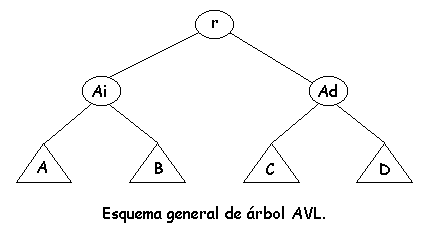
\includegraphics[width=8cm]{imagen_5.png}
\end{figure}